\documentclass[12pt]{article}
\usepackage[portuguese]{babel}
\usepackage{amsmath}
\usepackage{graphicx}
\usepackage{physics}
\newcommand{\numpy}{{\tt numpy}}   

\topmargin -.5in
\textheight 9in
\oddsidemargin -.25in
\evensidemargin -.25in
\textwidth 7in

\begin{document}
\textbf{• Problema 3.1} Encontre a entropia $S(E, V, N)$ de um gás ideal de $N$ partículas monoatômicas clássicas, com uma energia total fixa $E$, contido em uma caixa d-dimensional de volume $V$. Deduza a equação de estado deste gás, assumindo que $N$ é muito grande.

\textbf{Resposta:} O gás em questão é um sistema fechado e termicamente isolado, descrito pelo ensemble microcanônico. Sua entropia é definida, grosso modo, por $S = k \ln \Omega$, onde $\Omega$ é o número de microestados correspondentes à energia fixa $E$. No entanto, as coordenadas $q_i$ e os momentos $p_i$ $(i = 1, ..., dN)$ das partículas em um gás clássico podem assumir uma faixa contínua de valores, e algum cuidado é necessário para obter uma entropia bem definida. Para este fim, definimos $\Omega (E, V, N; \Delta E)$ como o volume de uma camada fina no espaço de fase correspondente a uma faixa estreita de energias entre $E$ e $E + \Delta E$. A definição precisa de entropia é então 
\[
S(E, V, N; \Delta E) = k \ln \left( \frac{\Omega(E, V, N; \Delta E)}{h^{dN} N!} \right)
\]

Nesta expressão, $h$ é uma constante arbitrária com as dimensões de (comprimento x momento), incluída para tornar o argumento do logaritmo adimensional. (Às vezes é conveniente identificar $h$ como a constante de Planck, para facilitar uma comparação entre gases clássicos e quânticos.) Como $\Delta E$ é pequeno, temos $\Omega (E, V, N; \Delta E) = \Delta E \sum (E, V, N)$, onde $\sum (E, V, N)$ é uma medida da área de uma superfície de energia constante. Consequentemente, tanto $h$ quanto $\Delta E$ contribuem para $S$ apenas com uma constante aditiva, que não tem significado físico. O fator $N!$ impõe a condição (às vezes referida como 'contagem correta de Boltzmann') de que estados que diferem apenas por uma das $N!$ permutações das $N$ partículas idênticas devem ser contados como o mesmo estado.

Para calcular $\Omega (E, V, N; \Delta E)$, expressamos como $\Omega = \Delta E \frac{\partial V}{\partial E}$, onde $V$ é o volume do espaço de fase correspondente a energias menores ou iguais a $E$. A Hamiltoniana de todo o sistema é
\[
\mathcal{H} = \sum_{i=1}^{dN} \frac{p_i^2}{2m}
\]
para partículas de massa m, então obtemos 
\[
\mathcal{V}(E, V, N) = \int_{\mathcal{H} \leq E} \prod_{i=1}^{dN} dp_i dq_i = V^N \int_{\sum p^2 \leq 2mE} d^{dN} p
\]
onde o fator $V^N $ é o resultado da integração sobre as coordenadas. A integral do momento é precisamente o volume de uma esfera $dN$-dimensional com raio $R = \sqrt{2mE}$  dado no apêndice A. Portanto, temos 
\[
\mathcal{V}(E, V, N) = \frac{V^N (2\pi m E)^{dN/2}}{(dN/2) \Gamma(dN/2)}
\]
e a entropia pode ser escrita como
 \[
 S(E, V, N; \Delta E) = k \Biggl\{ N \ln \left[ \frac{V (2 \pi m E)^{d/2}}{h^{d}} \right] - \ln \left[ \Gamma \left( \frac{dN}{2} \right) \right] - \ln(N!) + \ln \left( \frac{\Delta E}{E} \right) \Biggl\}
 \]
Para valores grandes de $N$, podemos usar a aproximação de Stirling $\ln(N!) \simeq N \ln N - N$ para obter \[
 S(E, V, N) \simeq Nk \biggl\{ \ln \left[ \frac{V }{N  } \left( \frac{ 4 \pi m E }{d N h^{2}}\right)^{\frac{d}{2}} \right] + \frac{d + 2}{2} \biggl\} 
 \]
 Observe que, nesta aproximação, a entropia é extensiva, uma vez que $S$/$N$ depende de $E$, $V$ e $N$ apenas nas combinações $V$/$N$ e $ E$/$N$.

Para obter a equação de estado, usamos a primeira lei da termodinâmica para escrever:
\[
P = T \left( \frac{\partial S}{\partial V} \right)_E = T \frac{Nk}{V}
\]
 o que fornece o resultado familiar $PV = NkT$. Também podemos encontrar a temperatura como uma função de $E, V$ e $N$ usando 
 \[
 \frac{1}{T} = \left( \frac{\partial S}{\partial E} \right)_V = \frac{dNk}{2E}
 \]
 Isso pode ser reorganizado para fornecer a relação usual $E = (d/2)NkT$ para a energia de um gás ideal clássico monoatômico. 

\textbf{• Problema 3.2} Considere um gás ideal de $N$ partículas monoatômicas quântico-mecânicas, com uma energia total fixa $E$, contido em uma caixa hipercúbica $d$-dimensional, de lado $L$. Para o caso em que $E$ é muito maior do que a energia do estado fundamental, obtenha uma expressão aproximada para a entropia$ S(E, V, N)$ e compare sua expressão com a entropia de um gás clássico. Nesta aproximação, e quando $N$ é grande, qual é a equação de estado do gás quântico? Qual é a probabilidade de encontrar uma partícula com momento $\vec{p}$ neste gás?
\textbf{Resposta:} Uma partícula livre de massa \textit{m} confinada a uma caixa hipercúbica tem autofunções de energia 
\[
\psi_{\mathbf{k}}(\mathbf{x}) = \left( \frac{2}{L} \right)^{d/2} \prod_{i=1}^{d} \sin(k_i x_i)
\]
onde, para que a função de onda se anule tanto em $x_i = 0$ quanto em $x_i = L$, os componentes do vetor de onda são restritos aos valores $k_i = n_i\pi/L$, onde cada $n_i$ é um inteiro positivo. A energia desse estado é $E_n = \hbar^2k^2/2m = (\pi^2\hbar^2/2mL^2) \sum n_i^2$. Uma autofunção de energia para o sistema de \textit{N} partículas é uma soma de produtos de \textit{N} dessas funções de partícula única que, para bósons, é simétrica ou, para férmions, é anti-simétrica, sob a troca de qualquer par de partículas. A energia total é 
\[
E = \sum_{i=1}^N \frac{\hbar^2 |\mathbf{k}_i|^2}{2m} = \sum_{j=1}^{dN} \frac{\hbar^2}{2m} k_j^2 = \epsilon \sum_{j=1}^{dN} n_j^2
\]
onde $\epsilon = \pi^2\hbar^2/2mL^2$. A entropia é $S(E, V, N) = k \ln[\Omega(E, V, N)]$, onde $\Omega(E, V, N)$ é o número de estados distintos com energia \textit{E}. Uma expressão exata para esse número é difícil de obter. Claramente, para bósons, $\Omega$ está relacionado ao número de conjuntos de inteiros $\{n_j\}$ cujos quadrados somam $E/\epsilon$. No caso de férmions, apenas aqueles conjuntos são permitidos que são consistentes com todas as partículas (que obedecem ao princípio de exclusão de Pauli) estando em diferentes estados quânticos. Uma boa resposta aproximada pode ser obtida quando \textit{E} é grande.

Se $E/\epsilon << 1$, então \textit{E} pode ser tratado como uma variável contínua e, se \textit{E} for muito maior do que a energia do estado fundamental, então muitos estados estão disponíveis, dos quais apenas uma pequena fração é proibida (para férmions) pelo princípio de exclusão.

O espaço $dN$-dimensional dos inteiros $\{n_i\}$ pode ser dividido em células de volume unitário, cada uma contendo exatamente um estado. Se permitirmos uma pequena incerteza em \textit{E}, então o número de estados com essa energia é, em uma boa aproximação, o número de células intersectadas por uma esfera de raio \(\sqrt{E/\epsilon}\), ou a área dessa esfera, que é $2\pi^{dN/2} (E/\epsilon)^{dN/2-1} / \Gamma(dN/2)$. Mais precisamente, desejamos incluir apenas aquele segmento da esfera para o qual todos os $n_j$ são positivos, que é uma fração $1/2^{dN}$ de toda a esfera, e também devemos dividir pelo número $N!$ de permutações das N partículas, que não contam como estados distintos. Desta forma, obtemos
\[
\begin{aligned}
\Omega(E, V, N) &= \frac{2 \pi^{dN/2}}{2^{dN} N! \Gamma(dN/2)} \left( \frac{E}{\epsilon} \right)^{dN/2 - 1} \\
&= \frac{V^N}{N! \Gamma(dN/2)} \left( \frac{2 \pi m E}{h^2} \right)^{\frac{dN}{2}} \frac{2 \epsilon}{E}
\end{aligned}
\]

onde $V = L^d$ e $h = 2\pi\hbar$. Note que, em contraste com a superfície de energia no espaço de fase considerada no problema anterior, a área de superfície necessária aqui é uma quantidade adimensional. Para partículas de spin s, haverá um fator adicional $(2s + 1)^N$ correspondente ao número de configurações de spin distintas.
Para a entropia de um gás de partículas de spin-0, temos
\[
S(E, V, N) = k \biggl \{  N \ln \left[ V \left( \frac{2 \pi m E}{h^2} \right)^{\frac{dN}{2}} \right] - \ln \left[ \Gamma \left( \frac{dN}{2} \right) \right] - \ln(N!) + \ln \left( \frac{2 \epsilon}{E} \right)  \biggl \}
\]
Exceto pelo último termo, que é insignificante quando $N$ é grande, isso é idêntico à expressão obtida no problema anterior para um gás clássico, mas aqui $h$ é realmente a constante de Planck. Obviamente, quando $N$ é grande, a equação de estado é a mesma que a de um gás clássico:$ P = T(\partial S/\partial V)_E = NkT/V$ ou $PV = NkT$. A ideia de determinar o momento de uma partícula específica em um gás quântico-mecânico é um tanto mal definida, uma vez que as partículas são, em princípio, indistinguíveis. No entanto, é razoável perguntar qual fração das partículas tem, em média, um momento em um determinado intervalo e isso pode ser vagamente interpretado como significando que a probabilidade de uma partícula selecionada aleatoriamente ter seu momento neste intervalo. Com essa ressalva, vamos primeiro perguntar pela probabilidade de que uma partícula selecionada aleatoriamente tenha energia $E_p = |\mathbf{p}|^2/2m$, enquanto a energia restante $E - E_p$ é distribuída de uma maneira não especificada entre as $N - 1$ outras partículas. Essa probabilidade é 
 \[
 \mathcal{P}(E_p) = \frac{\Omega(E_p, V, 1) \Omega(E - E_p, V, N - 1)}{N \Omega(E, V, N)}
 \]
 O numerador é o número de estados disponíveis para um par de sistemas, um consistindo de uma única partícula com energia $E_p$ e o outro de $N - 1$ partículas com energia total $E - E_p$. O fator $N^{-1}$ leva em conta o fato de que as $N$ maneiras de abstrair uma partícula levam a estados indistinguíveis, e $\mathcal{P}(E_p)$ é a razão entre o número resultante de estados distintos e o número de estados disponíveis para todo o sistema de $N$-partículas. Usando a expressão para $\Omega$ obtida acima, descobrimos que 
 \[
 \mathcal{P}(E_p) = \frac{\Gamma(dN/2)}{\Gamma((d(N-1))/2) \Gamma(d/2)} \cdot \frac{\epsilon}{E} \left( \frac{E_p}{E} \right)^{\frac{d}{2} - 1} \left( 1 - \frac{E_p}{E} \right)^{\frac{d(N-1)}{2} - 1}
 \]
Para apreciar o significado deste resultado, lembre-se que a energia é quantizada em unidades de $\epsilon$, mas que nossa aproximação para $\Omega$ é válida para grandes energias, que podem ser tratadas como continuamente distribuídas. Assim, para verificar que $\sum_{E_p} \mathcal{P}(E_p) = 1$, substituímos $\sum_{E_p}$por $\epsilon^{-1} \int_{0}^{E} dE_p$ e facilmente verificamos que a integral resultante é igual à unidade, usando o resultado padrão 
 \[
 \int_{0}^{1} dx \, x^{\alpha - 1} (1 - x)^{\beta - 1} = \frac{\Gamma(\alpha) \Gamma(\beta)}{\Gamma(\alpha + \beta)}
 \]
Além disso, nesta aproximação, o sistema é efetivamente isotrópico. É simples converter $\mathcal{P}(E_p)$ em uma distribuição de probabilidade para o momento usando 
 \[
 \int_{E_p \leq E'} d^d p \propto \int_{0}^{\sqrt{2mE}} p^{d-1} dp \propto \int_{0}^{E} E_p^{d/2 - 1} dE_p
 \]
 O fator $E_p^{d/2 - 1}$ em $\mathcal{P}(E_p)$ corresponde a este elemento de volume do espaço de momento. As constantes omitidas não são difíceis de encontrar, mas não são necessárias, já que já sabemos que a probabilidade está corretamente normalizada. Assim, temos 
 \[
 \mathcal{P}(\boldsymbol{p}) d^d p = \mathcal{N}(E) \left( 1 - \frac{E_p}{E} \right)^{\frac{d(N-1)}{2} - 1} d^d p
 \]
onde $\mathcal{N}(E)$ é um fator de normalização tal que $\int \mathcal{P}(\boldsymbol{p}) d^d p = 1$. É instrutivo avaliar essa densidade de probabilidade no espaço de momento no limite termodinâmico em que $N \rightarrow \infty$ com $E/N$ e $V/N$ fixos. De fato, como foi mostrado no problema 3.1, temos $\frac{E}{N} = \frac{d}{2} kT$; então, usando o fato de que$\lim_{N \to \infty} \left[ \left( 1 - \frac{x}{N} \right)^N \right] = e^{-x}$, descobrimos que 
 \[
 \mathcal{P}(\boldsymbol{p}) d^d p = \frac{e^{-\frac{E_p}{kT}} d^d p}{\int e^{-\frac{E_p}{kT}} d^d p}
 \]
 Esta expressão é válida para altas temperaturas, onde o gás quântico se comporta da mesma maneira que um gás clássico e é, obviamente, a expressão que escreveríamos imediatamente usando o ensemble canônico para um sistema em contato térmico com um banho de calor na temperatura $T$. Isso ilustra o fato de que os dois ensembles são equivalentes (para sistemas sem forças de longo alcance) no limite termodinâmico. 
 
\textbf{• Problema 3.4} Para uma coleção de $N$ osciladores harmônicos clássicos tridimensionais de frequência $\omega$ e energia total fixa $E$, calcule a entropia $S$ e a temperatura $T$. Discuta se os osciladores devem ser tratados como distinguíveis ou indistinguíveis.

\textbf{Resposta:} A Hamiltoniana do conjunto de $N$ osciladores harmônicos clássicos é 
\[
\mathcal{H} = \sum_{i=1}^{3N} \left( \frac{p_i^2}{2m} + \frac{1}{2} m \omega^2 q_i^2 \right)
\]
Precisamos encontrar o volume no espaço de fase dado por 
\[
\mathcal{V}(E, N) = \int_{\mathcal{H} \leq E} \prod_{i=1}^{3N} dp_i dq_i
\]
que pode ser calculado por meio das substituições 
\[
\begin{aligned}
p_i &= \sqrt{2m} x_i, & i &= 1, \dots, 3N \\
q_i &= \sqrt{\frac{2}{N}} \frac{x_{3N + i}}{m \omega}, & i &= 1, \dots, 3N
\end{aligned}
\]
Em termos dessas variáveis, a restrição de energia é $E = \sum_{i=1}^{6N} x_i^2$ e o volume é: 
\[
\mathcal{V}(E, N) = \left( \frac{2}{\omega} \right)^{3N} \int_D \prod_{i=1}^{6N} dx_i 
= \left( \frac{2}{\omega} \right)^{3N} \frac{\pi^{3N}}{3N \Gamma(3N)} E^{3N} 
\]
Aqui, $D$ é a região na qual a restrição é satisfeita, e a integral restante é o volume de uma esfera $6N$-dimensional com raio $R = \sqrt{E}$, que é dado no apêndice A. Para calcular a entropia (veja o problema 3.1 para detalhes), precisamos do volume $\Omega(E, N; \Delta E)$) da camada de energia de espessura $\Delta E$, que é 
\[
\Omega(E, N; \Delta E) = \Delta E \frac{\partial \mathcal{V}(E, N)}{\partial E} 
= \left( \frac{2}{\omega} \right)^{3N} \frac{\pi^{3N}}{\Gamma(3N)} E^{3N} \frac{\Delta E}{E} 
\]
Para N grande, usamos a aproximação de Stirling para obter
\[
S(E, N) = k \ln \left( \frac{\Omega}{h^{3N}} \right) 
\simeq 3Nk \left[ \ln \left( \frac{2 \pi E}{3 h \omega N} \right) + 1 \right]
\]

Ao obter esta expressão, consideramos os osciladores como distinguíveis e não inserimos um fator de $1/N!$ no primeiro logaritmo (veja a discussão abaixo). A temperatura é dada por

\[
\frac{1}{T} = \left( \frac{\partial S}{\partial E} \right)_N = \frac{3Nk}{E}
\]

Assim, a energia média por oscilador é $3kT$, de acordo com o teorema da equipartição.

Se os osciladores devem ser tratados como distinguíveis ou indistinguíveis depende da situação física que temos em mente. Nós os tratamos como distinguíveis (embora sejam idênticos), com o resultado de que a entropia é extensiva: $S/N$ é uma função apenas de $E/N$. Isso seria apropriado se, por exemplo, considerássemos os osciladores como modelando átomos em uma rede, assumindo que cada átomo oscila independentemente em torno de seu próprio sítio da rede. Podemos então distinguir os átomos pelos sítios aos quais estão ligados. Por outro lado, podemos considerar os osciladores como um gás de N partículas, todas ocupando um único poço de potencial. Nesse caso, qualquer posição no espaço poderia ser ocupada por qualquer uma das partículas e devemos tratá-las como indistinguíveis. A entropia seria diferente da calculada acima por uma quantidade $\Delta S = -Nk(\ln N - 1)$ e não seria extensiva. Como a diferença de entropia depende apenas de N, quantidades como a temperatura e o calor específico são as mesmas em ambos os casos. A questão da distinguibilidade é importante apenas quando consideramos a mudança no número de partículas. No caso de uma rede, isso só poderia ser feito tendo duas redes com a mesma energia média por partícula ($E_1/N_1 = E_2/N_2$). Temos então a liberdade de considerá-las como dois sistemas separados ou como um sistema combinado, e nossa escolha não deve ter consequências físicas. Isso é
\begin{figure}
    \centering
    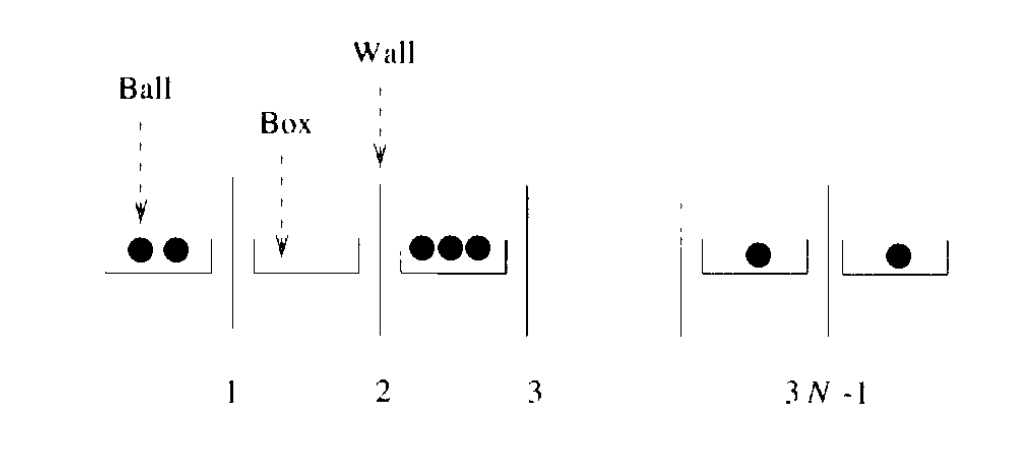
\includegraphics[width=0.5\linewidth]{image.png}
    \caption{\textbf{Figura 3.1:} Arranjo particular de M bolas em 3N caixas, (bbwwbbbw...), para contar o número de conjuntos de inteiros não negativos que somam M. }
    \label{fig:enter-label}
\end{figure}
De fato, é assim: como a entropia é extensiva, obtemos uma entropia total $S = S_1 + S_2$ em ambos os casos. Em contraste, o número de partículas em um gás pode ser alterado colocando o gás em contato com um reservatório de partículas, e a taxa de troca de partículas dependerá do número de partículas por unidade de volume no gás (e possivelmente de outros fatores). Portanto, há uma diferença física real entre ter $N$ poços de potencial, cada um contendo uma partícula, e ter um único poço contendo N partículas. Essa diferença é refletida na parte não extensiva da entropia $\Delta S$. 
 
\textbf{• Problema 3.5} Para uma coleção de $N$ osciladores harmônicos quânticos tridimensionais de frequência $\omega$ e energia total $E$, calcule a entropia $S$ e a temperatura $T$.

\textbf{Solução}

Para resolver este problema usando o conjunto micro-canônico, temos que contar todos os estados possíveis de todo o sistema com sua energia total fixa. A energia do sistema é
\begin{equation}
E = \sum^{3N}_{i=1} E_{l} = \sum^{3N}_{i=1} \left(n_{l}+\frac{1}{2} \right) \hbar \omega
\end{equation}
onde n, é o número de quanta de energia no oscilador i-ésimo $(n_{i} = 0,1, ... ,\infty)$. Podemos escrever isso como

\begin{equation}
\sum^{3N}_{i=1} n_{i} = \frac{E}{\hbar \omega} - \frac{3N}{2} \equiv M
\end{equation}

O número de estados possíveis é o número de conjuntos de inteiros não negativos $\{n_{i} \}$ que somam ate $M$. Este problema combinatório pode ser resolvido considerando os osciladores $3N$ como caixas, nas quais colocamos $M$ bolas indistinguíveis, representando os quanta de energia. Para contar o número de maneiras pelas quais isso pode ser feito, tratamos as caixas (osciladores) como distinguíveis e as imaginamos dispostas em uma fileira e separadas por paredes $3N — 1$, conforme ilustrado na figura 3.1. Um dado estado das bolas nas caixas pode ser visto como uma sequência de bolas e paredes. Por exemplo, a sequência $\{ bbwwbbbw... \}$ mostrada na figura corresponde a duas bolas na caixa 1, nenhuma bola na caixa 2, três bolas na caixa 3, e assim por diante. Se as bolas e as paredes fossem todas distinguíveis, o número total de arranjos desses objetos$ M + 3/V — 1$ seria $(M + 3N — 1)!$. Como as bolas são indistinguíveis umas das outras, e também as paredes, dividimos pelas permutações $M!$ das bolas e pelas permutações $(3N — 1)!$ das paredes para obter o número de arranjos distintos. Portanto, o número de estados possíveis distintos é

\begin{equation}
    \Omega(E,N) = \frac{(M+3N-1)!}{M!(3N-1)!}  ,
\end{equation}

substituindo  $M$

\begin{equation}
    \Omega(E,N) = \frac{(\frac{E}{\hbar \omega} + \frac{3N}{2-1})!}{\frac{E}{\hbar \omega} + \frac{3N}{2}!(3N-1)!}.
\end{equation}

A entropia é $S(E,N) = k ln[\Omega(E. N)]$. No limite termodinâmico, que $E,N \to \infty \quad \text{com} \quad \frac{E}{N}$ fixo, usamos a aproximação de Stirling para obter

\begin{equation}
    S(E, N) \approx NK \left[ \left(\frac{E}{N \hbar \omega} + \frac{3}{2} \right) ln\left(\frac{E}{N \hbar \omega} + \frac{3}{2} \right) - \left(\frac{E}{N \hbar \omega} - \frac{3}{2} \right) ln\left(\frac{E}{N \hbar \omega} - \frac{3}{2} \right)\right]
\end{equation}
Note que, como no problema 3.4, a entropia é extensa no limite termodinâmico, desde que os osciladores sejam distinguíveis. A temperatura é agora dada por
\begin{equation}
    \frac{1}{T} = \left(\frac{\partial S}{\partial E}\right)_{N} = \frac{k}{\hbar \omega} ln\left(\frac{E/N \hbar \omega + \frac{3}{2}}{E/N \hbar \omega - \frac{3}{2}} \right)
\end{equation}
Isso pode ser facilmente resolvido para $E$ em termos de $T$ e $N$, e obtemos
\begin{equation}
    E(T, N) = \frac{3}{2} N \hbar \omega coth\left(\frac{\hbar \omega}{2 k T}\right),
\end{equation}
que é o resultado que seria obtido do conjunto canônico. Em altas temperaturas, $kT \ll \hbar \omega$ ou, equivalentemente, quando $E \ll 3N\hbar \omega$. recuperamos o resultado clássico do problema 3.4, a saber, $E \approx 3NkT$.

\textbf{• Problema 3.6} Usando o ensemble micro-canônico, calcule a energia livre de Helmholtz $F(T, N)$ como uma função da temperatura para um sistema de $N$ partículas idênticas, mas distinguíveis, cada uma das quais possui dois níveis de energia. Explore os limites $T \rightarrow 0$ e $T \rightarrow \infty$ da energia, da entropia e dos números de ocupação.

Mostre que a entropia máxima (mínima) corresponde à informação mínima (máxima) sobre o sistema. Quantos bits de informação são perdidos se o sistema evolui de um estado inicial de temperatura zero para um estado final de temperatura infinita? Qual é a temperatura mais alta na qual este sistema pode existir?

\textbf{Solução}

Vamos supor que cada partícula pode ter uma energia $\pm \epsilon$, e que partículas $n_{+}$ têm energia $+\epsilon$. Obviamente, o número de partículas com energia $-\epsilon$ é $n_{-} = N - n_{+}$ e, se a energia total é $E$, então $n_{\pm} = (N \pm E/\epsilon)/2$. O número de microestados com energia $E$ é apenas o número de maneiras pelas quais $n_{+}$ (ou $n_{-}$) partículas podem ser escolhidas de N, temos que
\begin{equation}
\Omega(E, N) =  \begin{bmatrix}
N   \\
n_{+}  \end{bmatrix}  = \frac{N!}{n_{+}!(N - n_{+})!}
\end{equation}
Como de costume, obtemos uma forma compacta para a entropia no limite termodinâmico. Neste caso, tomamos $N$, $n_{+}$ e $n_{-}$ todos como grandes. Usando a aproximação de Stirling e a definição
\begin{equation}
x = \frac{n_{+}}{N} = \frac{1}{2}\left(1 + \frac{E}{N \epsilon} \right)
\end{equation}
nós descobrimos que
\begin{equation}
S(E,N) = k ln \Omega \approx - Nk\left[xln + (1-x)ln(1-x) \right]
\end{equation}
e note que isso é extenso, desde que as partículas sejam distinguíveis (cf. problemas 3.4 e 3.5). A temperatura é dada por
\begin{equation}
\frac{1}{T} = \left(\frac{\partial S}{\partial E} \right)_{N} = \frac{1}{2 N \epsilon} \left(\frac{\partial S}{\partial X} \right)_{N} = \frac{k}{2 \epsilon} ln \left( \frac{1-x}{x}\right)
\end{equation}
e essa relação pode ser invertida para produzir
\begin{equation}
    x = (e^{\frac{2 \epsilon}{kT} + 1}) ] \qquad E(T, N) = -N \epsilon tanh\left(\frac{\epsilon}{kT} \right)
\end{equation}
Agora é uma questão simples calcular a energia livre de Helmholtz;
\begin{equation}
    F(T, N) = E(T ,N) - TS(T, N) = -N\epsilon -NkTln\left(1+e^{\frac{2 \epsilon}{kT} + 1}\right)
\end{equation}
É claro que esse resultado também seria obtido a partir do conjunto canônico:
\begin{equation}
    e^{-\frac{F}{kT}} = \prod_{i=1}^{N} \sum_{E_{i} = \pm \epsilon} e^{\frac{-E_{i}}{kT}} = e^{\frac{N \epsilon}{kT}} \left(1 + e^{\frac{-2\epsilon}{kT}} \right)^{N}
\end{equation}
No limite $T \to 0$, encontramos que $x \to 0$, então $n_{+}(0, N) = 0$, $ n_{-}(0, N) = N$, $E(0, N) = -N \epsilon$ e $S(0, N) = 0$. Claramente, todas as partículas têm sua menor energia e a entropia desaparece porque há apenas um estado com essa energia mínima. Como $x$ deve estar entre zero e um, $S$ não pode ser negativo, então $S = 0$ é seu valor mínimo. Precisamos de $N$ bits de informação para especificar esse estado.
No limite $T \to \infty$, obtemos $x \to \frac{1}{2}$, então $n_{+}(\infty,  N) = n_{-} = (\infty, N) = \frac{N}{2}$. $E(\infty, N) = 0$ e $S(\infty, N) = N k ln2$. Intuitivamente, é bastante claro que esse estado, no qual os níveis de energia são igualmente ocupados, tem o maior grau possível de desordem. De fato, é fácil verificar que $S$ atinge seu valor máximo quando $x = \frac{1}{2}$ Como cada partícula tem probabilidades iguais de estar em qualquer um dos seus dois níveis de energia, o conteúdo de informação desse estado é zero. Consequentemente, A' bits de informação são perdidos se o sistema for aquecido de $T = 0$ a $T = \infty$. Isso pode ser confirmado usando a relação entre informação e entropia:
\begin{equation}
\Delta I = \frac{S(0, N) - S(\infty, N)}{k ln 2} = N.
\end{equation}
A energia máxima que o sistema pode conter é, é claro,$ E_{max} = +N\epsilon$, que corresponde a , $x = 1$ ou a $T = 0$. Conforme discutido no problema 2.2, a faixa de temperaturas disponíveis para o sistema é melhor compreendida em termos do parâmetro $\beta = 1/kT$. A menor temperatura possível $T=0$ corresponde ao maior valor possível de $\beta$. ou seja, $\beta = \infty$. onde $E = - N \epsilon$ e $x = 0$. À medida que $E$ é aumentado, $x$ aumenta suavemente até zero. À medida que $E$ se aproxima de $E_{max}$, $x$ se aproxima de seu valor máximo de unidade, enquanto $\beta$ se aproxima de seu valor mínimo de $-\infty$. Isso corresponde a $T$ aumentando em direção a zero por meio de valores negativos.

\textbf{• Problema 3.9} Considere um sistema de $N$ osciladores harmônicos quântico-mecânicos que não interagem em três dimensões. Calcule a função de partição canônica do sistema $Z(T, N)$. Verifique se a mesma resposta é obtida considerando o sistema como consistindo de:

(a) $3N$ osciladores unidimensionais ou

(b) $N$ osciladores tridimensionais.

\textbf{Solução:}\\

O hamiltoniano para um oscilador de três dimensões é simplesmente a soma dos hamiltonianos para três osciladores de uma dimensão, então nós estamos livres em considerar o sistema como uma coleção de $3N$-osciladores de uma dimensão ou de $N$ osciladores de três dimensões. Em ambos os casos, já que os osciladores não interagem, a função de partição $Z(T,N)$ é o produto de funções de partição parar osciladores individuais:

\begin{equation}
Z(T,N) = \prod_{i=1}^{M} Z_i(T) = \prod_{i=1}^{M} \left(\sum_{n_i = 0}^\infty g(n_i) e^{-\beta E_i(n_i)}\right)
\end{equation}

Onde $M$ é $3N$ ou $N$ e, para o i-ésimo oscilador, $g(n_i)$ é a degenerescência do nível de energia indicado por $n_i$.

\mathbf{a)} $3N$ osciladores de uma dimensão:\\

Para um oscilador de uma dimensão de frequência angular $\omega$, os níveis de energia são $E_i(n_i) = \left(n_i +\frac{1}{2}\right)\hbar\omega$ e são não degenerados, então $g(n_i) = 1$. Logo,

\begin{equation}
    Z(T,N) = \prod_{i=1}^{3N} \left(\sum_{n_i =0}^{\infty} e^{-\beta\hbar\omega(n_i+\frac{1}{2})}\right) = \left(e^{-\frac{\beta\hbar\omega}{2}}\sum_{n_i=0}^{\infty} e^{-\beta\hbar\omega n} \right)^{3N} .
\end{equation}

Usando a expansão binomial,

\begin{equation}
    L(q) \equiv \sum_{n=0}^{\infty} = \frac{1}{1-q}
\end{equation}

ao qual é válido para $q<1$ e (com $q=e^{\beta\hbar\omega}$) nós obtemos a resposta

\begin{equation}
Z(T,N) = \left(\frac{e^{-\frac{\beta\hbar\omega}{2}}}{1-e^{-\beta\hbar\omega}}\right)^{3N}.
\end{equation}

\textbf{b)} $N$ osciladores de 3 dimensões:\\

Os níveis de energia de um oscilador de três dimensões são $E_i(n_i) = (n_i + \frac{3}{2})\hbar\omega$. A degenerescência de um destes níveis é o número de conjuntos de três inteiros não negativos que adicionam para $n_i$. Isso pode ser encontrado, por exemplo, pelo método sugerido na solução para o problema 3.5 e é dado por 

\begin{equation}
    g(n_i) = \frac{(n_i + 2)!}{2!n!} = \frac{1}{2}n_i^2 + \frac{3}{2} n_i + 1.
\end{equation}

Logo,

\begin{equation}
    Z_i = e^{-\frac{\beta\hbar\omega}{2}}\sum_{n_i=0}^{\infty}\left(\frac{1}{2}n_i^2+\frac{3}{2}n_i+1\right)e^{-\beta\hbar\omega n}.
\end{equation}

As somas podem ser resolvidas usando a formula anterior, junto com:

\begin{align}
    \sum_{n=0}^\infty n q^n &= q \dv{q}[L(q)]  =\frac{q}{(1-q)^2}\\
    \sum_{n=0}^\infty n^2q^n &= \left(q \dv{q}\right)^2[L(q)] = \frac{q(1+q)}{(1-q)^3}.
\end{align}

A função de partição total é então encontrado

\begin{equation}
    Z(T,N) = \left[e^{-\frac{3\beta\hbar\omega}{2}}\left(\frac{1}{2}\frac{q(1+q)}{(1-q)^3} + \frac{3}{2}\frac{q}{(1-q)^2}+\frac{1}{1-q}\right)\right].
\end{equation}

Manipulando,

\begin{align}
    \frac{1}{2}\frac{q(1+q)}{(1-q)^3} + \frac{3}{2}\frac{q}{(1-q)^2}+\frac{1}{1-q} &= \frac{1}{2}\frac{q(1+q)}{(1-q)^3}+\frac{q(1-q)}{(1-q)^3} + \frac{2}{2}\frac{(1-q)^2}{(1-q)^3}\\
    &= \frac{1}{2(1-q)^3}\left(q(1+q) + 3q(1-q) + 2(1-q)^2\right)\\
    &=\frac{1}{2(1-q)^3}(2)\\
    &=\left(\frac{1}{1-q}\right)^3.
\end{align}

Retornando para a função de partição, temos

\begin{equation}
    Z(T,N) = \left(\frac{e^{-\frac{\beta\hbar\omega}{2}}}{1-e^{-\beta\hbar\omega}}\right)^{3N}.
\end{equation}

\textbf{• Problema 3.18} A uma dada temperatura, a diferença entre os calores específicos de um gás ideal diatômico e um gás monoatômico é devida em parte à energia rotacional das moléculas diatômicas. Um rotor quântico rígido possui níveis de energia $E_\text{rot}(l)$ com degenerescência $g(l)$ dada por 
\[
E_{\text{rot}}(l) = l(l+1) \frac{\hbar^2}{2I} \qquad g(l) = 2l + 1 \qquad l = 0, 1, 2, ...
\]
 onde $l$ é o momento de inércia.
 
(a) Encontre a função de partição canônica de um gás de N moléculas diatômicas que não interagem.

(b) Avalie o calor específico deste gás em altas temperaturas e nas temperaturas mais baixas em que o movimento rotacional das moléculas dá uma contribuição significativa.

 \textbf{Solução:}
 
(a) Como as moléculas não interagem, podemos expressar a função de partição canônica como $Z(T, V, N) = \frac{Z^{N}_{1}}{N!}$, onde $Z_{1}$ é a função de partição para uma única molécula. O hamiltoniano quântico para cada molécula é a soma de um termo translacional e um termo rotacional e pode ser diagonalizado na base do espaço de Hilbert formado pelos autoestados simultâneos $|p, l\rangle$ de momento e momento angular. Temos então
\begin{equation}
\langle p,l| H |p,l\rangle = \frac{|p|^{2}}{2m} + l(l+1)\frac{\hbar^{2}}{2I}
\end{equation}
e a função de partição $Z_{1}$ por ser escrita como um produto das contribuições translacional e rotacional, definidas
\begin{equation}
    Z_{trans} = \frac{B}{h^{3}} \int d^{3} p e^{- \beta |p|^{2}/2m} = \frac{V}{\lambda^{3}}
\end{equation}
\begin{equation}
Z_{rot} = \sum^{\infty}_{l=0} g(l)e^{- \beta l(l+1)\hbar^{2}/2I}
\end{equation}
onde o comprimento de onda térmico de Broglie é $\lambda = (h^{2}/2mkT)^{1/2}$ e a degenerescência é $ g(l) = 2l + 1$. A parte translacional $Z_{trans}$ foi aproximada por sua versão clássica porque, em todas as situações práticas, o espaçamento do nível de energia é muito menor que $kT$, e a soma sobre esses níveis pode ser substituída por uma integral (veja o problema 3.11). Assim, obtemos
\begin{equation}
Z(T, V, N) = \frac{1}{N!} \left(\frac{V}{\lambda^{3}}\sum^{\infty}_{l=0}g(l)e^{- \beta l(l+1)\hbar^{2}/2I}\right)
\end{equation}
A soma restante pode ser avaliada analiticamente apenas nos limites de altas ou baixas temperaturas.

(b) Em temperaturas suficientemente altas, poderíamos esperar que o espaçamento dos níveis de energia rotacional se tornasse suficientemente pequeno comparado com $kT$ que a soma acima poderia ser substituída por uma integral, correções para essa aproximação se tornando significativas conforme a temperatura é reduzida. Essa expectativa pode ser tornada precisa por meio da fórmula de Euler-Maclaurin (dada no apêndice A) que é
\begin{equation}
\sum^{\infty}_{k=0} f(k) = \int^{\infty}_{0} f(k)dk + \frac{1}{2}f(0) - \frac{1}{12}f^{\prime}(0) + \frac{1}{720}f^{\prime \prime \prime}(0) - (...).
\end{equation}

Nesta forma, a fórmula é válida para funções suaves $f(k)$ que desaparecem, e todas as derivadas desaparecem, como $k \rightarrow \infty$, como é frequentemente o caso em aplicações à mecânica estatística. Claro, esta fórmula é útil apenas em circunstâncias onde todos, exceto alguns termos da série, podem ser negligenciados. No caso presente, vamos definir $ \theta =\hbar^{2}/2Ik$ e $f(l) = (2l+1) e^{-l(l+1)\theta/T}$. A série de Euler-Maclaurin pode ser convertida em uma expansão de série de potências de $Z_{rot}$ em potências de $\theta/T$, das quais precisamos manter apenas alguns termos quando $T \gg \theta$. No entanto, essas duas séries não concordam termo por termo. De fato, vamos expandir $f(l)$ em potências de $\theta/T$:
\begin{align}
Z_{rot} &= \int^{\infty}_{0} f(l)dl + \frac{1}{2}f(0) - \frac{1}{12}f^{\prime}(0) + \frac{1}{720}f^{\prime \prime \prime}(0) - (...) \\
&= \frac{T}{\theta} + \frac{1}{3} + \frac{1}{15}\frac{\theta}{T} + O\left[\left(\frac{\theta}{T} \right)^{2} \right].
\end{align}
A energia interna e o calor específico são então dados por
\begin{align}
    U &= -N\left(\frac{\partial(lnZ_{trans})}{\partial \beta} +\frac{\partial(lnZ_{rot})}{\partial \beta} \right) \\
    &= \frac{5}{2}NKT \biggl\{ 1 - \frac{2 \theta}{15 T} - \frac{2}{225}\left( \frac{\theta}{T}\right)^{2} + O \left[\left(\frac{\theta}{T} \right)^{3} \right] \biggl\}\\
    C_{V} &= \left( \frac{\partial U}{\partial T} \right)_{V} = \frac{5}{2}NK \biggl\{ 1 +  \frac{2}{225}\left( \frac{\theta}{T}\right)^{2} + O \left[\left(\frac{\theta}{T} \right)^{3} \right] \biggl\}
\end{align}
Claro, o limite de alta temperatura $C_{V} \approx \frac{5NK}{2}$ concorda com o teorema clássico da equipartição. Em baixas temperaturas $T « \theta$, termos sucessivos da soma sobre $l$ diminuem rapidamente, e precisamos manter apenas alguns deles. Mantendo apenas os dois primeiros termos, obtemos
\begin{equation}
    Z_{rot} = 1 + 3e^{-2\theta/T}+ ( . . . )
\end{equation}
e
\begin{equation}
    C_{V} = \frac{3}{2}NK + 12NK \left(\frac{\theta}{T}\right)\left(e^{-2\theta/T}+ ( . . . )\right)
\end{equation}
O segundo termo é a contribuição rotacional. Ela desaparece quando $T \to 0$, de acordo com a terceira lei da termodinâmica, e este é um efeito mecânico-quântico (por exemplo, problema 3.11). O primeiro termo é devido ao movimento translacional e concorda com o teorema da equipartição clássica quando apenas os graus de liberdade translacionais são levados em conta. Ela não desaparece em $T = 0$, embora o resultado totalmente mecânico-quântico necessário em temperaturas extremamente (e impraticavelmente) baixas desapareça (problema 3.11).
Leitores que não estão familiarizados com a fórmula de Euler-Maclaurin podem gostar de obtê-la por si mesmos. O seguinte sugere um método simples (que, no entanto, não prova que a série realmente converge para o resultado desejado). Primeiro, expresse a integral como
\begin{align}
\int^{\infty}_{0} f(x) dx &= \sum_{k=o}^{\infty} \int_{0}^{1} f(k+x)dx \\
&= \sum_{k=o}^{\infty} \int_{0}^{1} \left(f(k) + x{f^{\prime}}(k)+\frac{x^{2}{f^{\prime \prime}}(k)}{2} + (...)\right)dx \\
&= \sum_{k=o}^{\infty} \left(f(k) + 
\frac{f^{\prime}(k)}{2}+\frac{{f^{\prime \prime}}(k)}{6} + (...) \right)
\end{align}
Assumindo que
\begin{equation}
    \sum_{k=o}^{\infty} = \int_{0}^{\infty} f(x)dx + a_{0}f(0) + a_{1}{f^{\prime}}(0) + a_{2}{f^{\prime \prime}}(0) + (. . .)
\end{equation}
e que as somas de ${f^{\prime}}(k)$, ${f^{\prime \prime}}(k)$, etc, podem ser expressas da mesma forma, com os mesmos coeficientes $a_{i}$. Substitua essas expressões no primeiro resultado. A integral de $f(x)$ cancela. Assumindo que $f(\infty) = {f^{\prime}}(\infty) = (• • •) = 0$, a integral de ${f^{\prime}}(x)$ é $-f(0)$, a integral de ${f^{\prime \prime}}(x)$ é $-{f^{\prime}}(0)$ e assim por diante. Definindo os coeficientes de $f(0)$, ${f^{\prime}}(0)$, etc, iguais a zero, obtém-se uma sequência de equações que podem ser resolvidas para as constantes $a_{i}$.
\end{document}